\documentclass[10pt,french]{article}

\input preambule_2013

%-------------------------------------------------------------------------------------------------------
% Représenter différentes étapes d'une construction géométrique :
%-------------------------------------------------------------------------------------------------------

%-------------------------------------------------------------------------------------------------------
% Définition de longueur utile pour la commande \film ci-après
%-------------------------------------------------------------------------------------------------------

\newlength{\epais}
\setlength{\epais}{12pt}
\newlength{\maigre}
\setlength{\maigre}{0.2pt}
\newlength{\normal}
\setlength{\normal}{\arrayrulewidth}

%-------------------------------------------------------------------------------------------------------
% Définition de nouveaux types de séparateur de colonne
%-------------------------------------------------------------------------------------------------------

\newcolumntype{I}{!{\vrule width \epais}}
\newcolumntype{i}{!{\vrule width 10\maigre}}

%-------------------------------------------------------------------------------------------------------
% Commande pour les gros carrés noirs
%-------------------------------------------------------------------------------------------------------

\newcommand*\Hepais[1]{%
  \noalign{\global\setlength{\arrayrulewidth}{0.35\epais}}%
  \cline{#1}%
  \noalign{\global\setlength{\arrayrulewidth}{0.5\normal}}%
}

%-------------------------------------------------------------------------------------------------------
% Commande \film
% Syntaxe à utiliser : \film{Figure 1}{Figure 2}{Figure 3}{Texte 1}{Texte 2}{Texte 3}
%-------------------------------------------------------------------------------------------------------

\newcommand{\film}[6]{
\begin{tabular}{i*{18}{cI}} % un séparateur vertical de type "i" suivi de 18 colonnes "c"  avec un séparateur vertical de type "I" à chaque fois.
  \Hepais{1-18}
        &&&&&&&&&&&&&&&&&\\
  \Hepais{1-18}
        \multicolumn{6}{ici}{} & \multicolumn{6}{c}{} & \multicolumn{6}{ici}{}\\

        \multicolumn{6}{ici}{\begin{minipage}[c]{{0.2\linewidth}}\centering{#1}\end{minipage}}
            &
        \multicolumn{6}{c}{\begin{minipage}[c]{{0.2\linewidth}}\centering{#2}\end{minipage}}
            &
        \multicolumn{6}{ici}{\begin{minipage}[c]{{0.2\linewidth}}\centering{#3}\end{minipage}}\\

        \multicolumn{6}{ici}{} & \multicolumn{6}{c}{} & \multicolumn{6}{ici}{}\\

    \Hepais{1-18}
        &&&&&&&&&&&&&&&&& \\
    \Hepais{1-18}
        \multicolumn{6}{c}{} & \multicolumn{6}{c}{} & \multicolumn{6}{c}{}\\

        \multicolumn{6}{c}{\begin{minipage}[t]{{0.2\linewidth}}#4\end{minipage}}
            &
        \multicolumn{6}{c}{\begin{minipage}[t]{{0.2\linewidth}}#5\end{minipage}}
            &
        \multicolumn{6}{c}{\begin{minipage}[t]{{0.2\linewidth}}#6\end{minipage}}
\end{tabular}
}


\begin{document}


\begin{center}
    \small
        \film%
%------------FIGURE 1
            {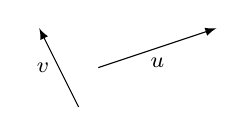
\begin{tikzpicture}[scale=0.5,>=latex]
                \draw[->] (0,0) -- ++(3,1) node[midway,below] {\footnotesize$\vect u$};
                \draw[->] (-0.5,-1) -- ++(-1,2) node[midway,left] {\footnotesize$\vect v$};
            \end{tikzpicture}}
%------------FIGURE 2
            {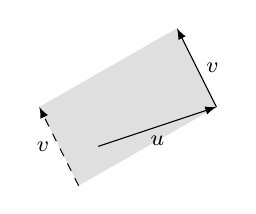
\begin{tikzpicture}[scale=0.5,>=latex]
                \fill[color=lightgray!50] (-0.5,-1) -- (3,1) -- (2,3) -- (-1.5,1) -- cycle;
                \draw[->] (0,0) -- ++(3,1) node[midway,below] {\footnotesize$\vect u$};
                \draw[->,dashed] (-0.5,-1) -- ++(-1,2) node[midway,left] {\footnotesize$\vect v$};
                \draw[->] (3,1) -- ++(-1,2) node[midway,right] {\footnotesize$\vect v$};
            \end{tikzpicture}}
%------------FIGURE 3
            {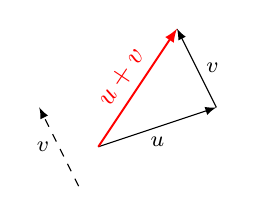
\begin{tikzpicture}[scale=0.5,>=latex]
                \draw[->] (0,0) -- ++(3,1) node[midway,below] {\footnotesize$\vect u$};
                \draw[->,dashed] (-0.5,-1) -- ++(-1,2) node[midway,left] {\footnotesize$\vect v$};
                \draw[->] (3,1) -- ++(-1,2) node[midway,right] {\footnotesize$\vect v$};
                \draw[->,red,line width=0.7pt] (0,0) -- ++(2,3) node[midway,above,sloped] {$\vect{u}+\vect{v}$};
            \end{tikzpicture}}
%------------TEXTE 1
            {\textbf{\'Etape 1 :} On veut représenter $\vect u + \vect v$.}
%------------TEXTE 2
            {\textbf{\'Etape 2 :} On dessine un représentant de $\vect v$ à l'extrémité de $\vect u$.}
%------------TEXTE 3
            {\textbf{\'Etape 3 :} On utilise la relation de Chasles.}
\end{center}

\end{document}

